\chapter{Exploratory Analysis}
In this chapter, I will copy the training  set to an exploratory set and 
work with it, because the exploratory analysis may require some data 
transformations, however I want to keep the training set untouched.

I will explore each attribute and its characteristics. Here is a list of
dataset attributes:
\begin{itemize}
	\item PassengerId
    \item Survived
    \item Pclass (page \pageref{section:Pclass})
    \item Name (page \pageref{section:Name})
    \item Sex (page \pageref{section:Sex})
    \item Age (page \pageref{section:Age})
    \item SibSp (page \pageref{section:SibSp})
    \item Parch (page \pageref{section:Parch})
    \item Ticket (page \pageref{section:Ticket})
    \item Fare (page \pageref{section:Fare})
    \item Cabin (page \pageref{section:Cabin})
    \item Embarked (page \pageref{section:Embarked})
\end{itemize}

I won't consider \textbf{"PassengerId"} and \textbf{"Survived"} attribures.
\textbf{"PassengerId"} attribute contains 891 passenger's IDs (see section 
\hyperref[section:first_rows]{First rows of the dataset} and table 
\ref{table:unique_values}), which won't help in building a model.
\textbf{"Survived"} attribute is a target. A passenger survived if their 
\textbf{"Survived"} attribute is 1, else the passenger drowned 
(\textbf{"Survived"} attribute is 0). Figure \ref{number_of_survivors}
shows numbers of survived and drowned passengers in whole dataset.


\section{Pclass} \label{section:Pclass}

\subsection{Description}
The \textbf{Pclass} attribute contains information about socio-economic
status of the passenger:
\begin{itemize}
    \item 1st = Upper
    \item 2nd = Middle
    \item 3rd = Lower
\end{itemize}

The table \ref{table:pclass_head} contains excerpt from attribute's column.
The table \ref{table:pclass_characteristics} contains the attribute 
characteristics.

\begin{table}[!ht]
    \centering
    \caption{Excerpt from the \textbf{Pclass} column}
    \begin{tabular}{|l|l|l|l|l|l|}
        \hline
        \textbf{Index}     & 788 & 347 & 629 & 734 & 106 \\ \hline
        \textbf{Attribute} & 3   & 3   & 3   & 2   & 3   \\ \hline
    \end{tabular}
    \label{table:pclass_head}
\end{table}

\begin{table}[!ht]
    \centering
    \caption{Attribute characteristics}
    \begin{tabular}{|l|l|}
        \hline
        \textbf{Characteristic}   & \textbf{Value} \\ \hline
        Type                      & category       \\ \hline
        Number of values          & 712            \\ \hline
        Number of non-null values & 712            \\ \hline
        Number of unique values   & 3              \\ \hline
        Most frequent value       & 3              \\ \hline
    \end{tabular}
    \label{table:pclass_characteristics}
\end{table}

The table \ref{table:pclass_value_counts} contains the number of occurrences of
each value.

\begin{table}[!ht]
    \centering
    \caption{Number of occurrences of each value}
    \begin{tabular}{|l|l|}
        \hline
        \textbf{Value} & \textbf{Number} \\ \hline
        3              & 402             \\ \hline
        1              & 172             \\ \hline
        2              & 138             \\ \hline
    \end{tabular}
    \label{table:pclass_value_counts}
\end{table}

\subsection{Analysis}
Let's estimate the number of passengers of each class in the exploratory
set. The figure \ref{pic:pclass_count} illustrates this estimation.

\begin{figure}[!ht]
    \centering
    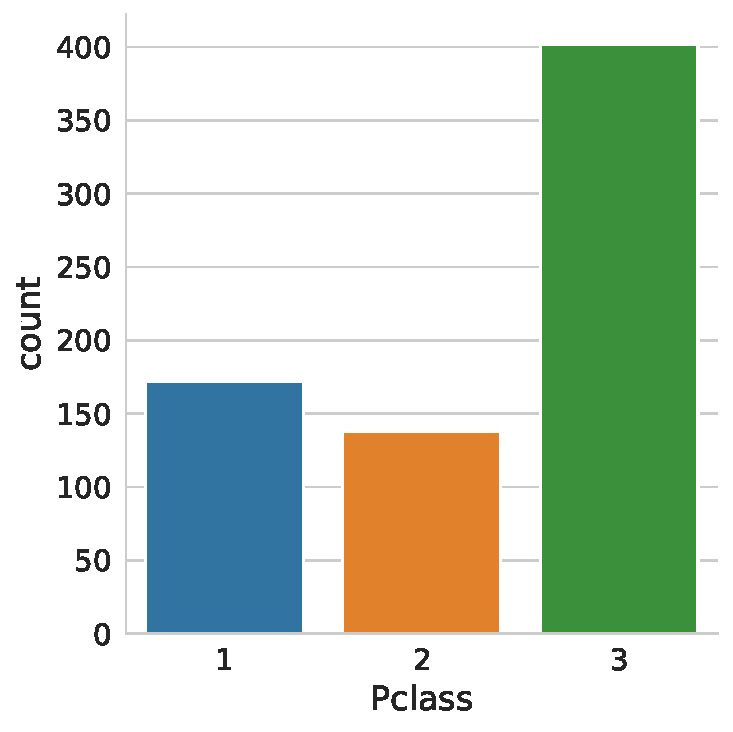
\includegraphics[width=0.5\textwidth]{pclass_count}
    \caption{Number of passengers in each \textbf{Pclass}}
    \label{pic:pclass_count}
\end{figure}

The figure \ref{pic:pclass_survived_entire_dataset} shows the proportions
of survived passengers for each \textbf{Pclass} in the exploratory set.

\begin{figure}[!ht]
    \centering
    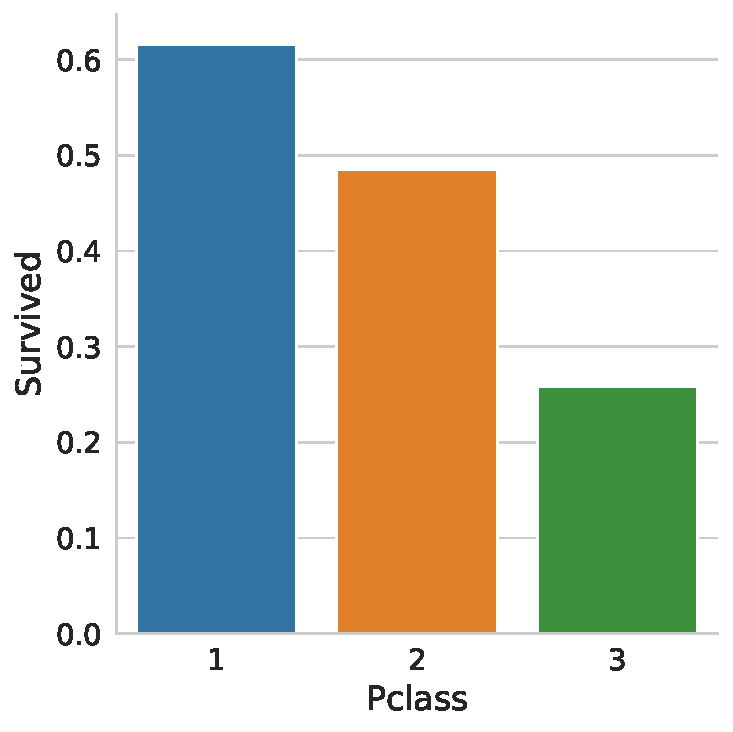
\includegraphics[width=0.5\textwidth]{pclass_survived_entire_dataset}
    \caption{Proportion of survived passengers in each \textbf{Pclass}}
    \label{pic:pclass_survived_entire_dataset}
\end{figure}

It looks like there were more passengers of the lower socio-economic class 
(\textbf{Pclass}=3), but they had less chance of surviving. \textbf{Pclass}
is a class of the ticket, so it contains information about the location 
of the passenger's cabin. It is known that the cabins of passengers with 
low socio-economic status were located on lower decks, that is, further 
from the lifeboats, this explains why there are fewer survivors among them
\cite{titanic-wikipedia}.

Finally, let's check the proportion of women among the survivors of each
\textbf{Pclass}. Figure \ref{pic:pclass_survived_gender} show these 
proportions.

\begin{figure}[!ht]
    \centering
    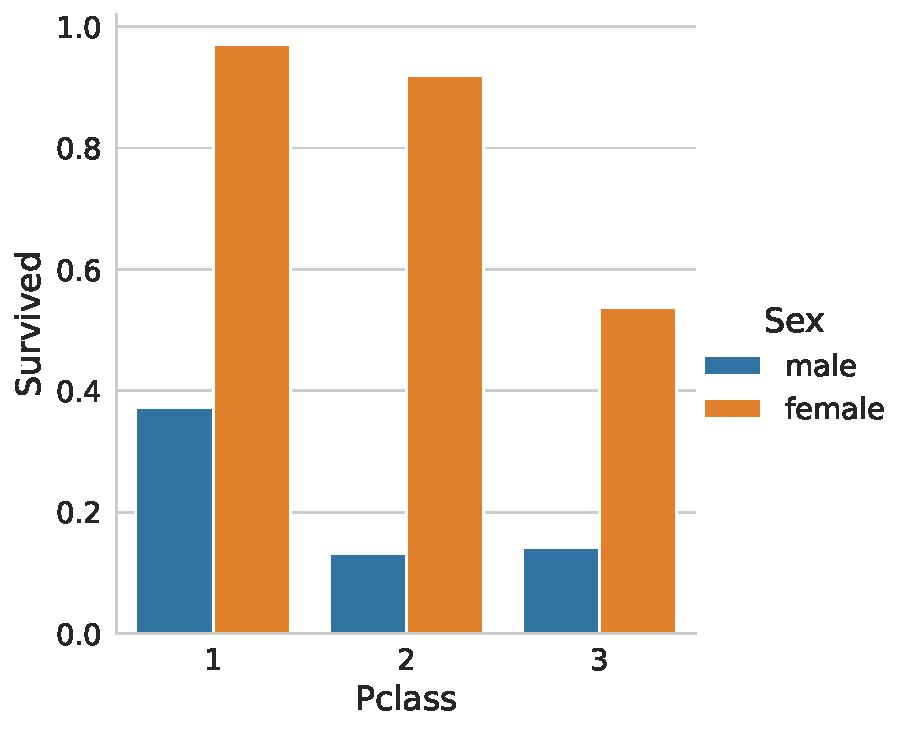
\includegraphics[width=0.5\textwidth]{pclass_survived_gender}
    \caption{Proportion of survived passengers of eache gender in each \textbf{Pclass}}
    \label{pic:pclass_survived_gender}
\end{figure}

More women than men survived in each \textbf{Pclass}.


\section{Name} \label{section:Name}
\subsection{Description}
The \textbf{Name} attribute contains names of passengers, and it contains
712 unique values in the exploratory dataset, so each value occurs only
once. The table \ref{table:name_column_excerpt} shows the exerpt from 
this column. The table \ref{table:name_characteristics} contains the 
attribute characteristics.

\begin{table}[!ht]
    \centering
    \caption{Excerpt from the \textbf{Name} column}
    \begin{tabular}{|l|l|}
        \hline
        \textbf{Index} & \textbf{Name}                             \\ \hline
        788            & Dean, Master. Bertram Vere                \\ \hline
        347            & Davison, Mrs. Thomas Henry (Mary E Finck) \\ \hline
        629            & O'Connell, Mr. Patrick D                  \\ \hline
        734            & Troupiansky, Mr. Moses Aaron              \\ \hline
        106            & Salkjelsvik, Miss. Anna Kristine          \\ \hline
    \end{tabular}
    \label{table:name_column_excerpt}
\end{table}

\begin{table}[!ht]
    \centering
    \caption{Attribute characteristics}
    \begin{tabular}{|l|l|}
        \hline
        \textbf{Characteristic}   & \textbf{Value} \\ \hline
        Type                      & object         \\ \hline
        Number of values          & 712            \\ \hline
        Number of non-null values & 712            \\ \hline
        Number of unique values   & 712            \\ \hline
    \end{tabular}
    \label{table:name_characteristics}
\end{table}

\subsection{Analysis}
There seems to be a useful pattern. Each name contains a title, such as 
"Mrs." or "Master.". The title may contain information about gender, 
socio-economic status, age, etc. 

Let's create new feature \textbf{Title} containing the title from each 
name and count how many times each title occurs in the exploratory set. 
The results is shown in the table \ref{table:titles_number} and figure 
\ref{pic:title_count}.

\begin{table}[!ht]
    \centering
    \caption{Number of occurrences of each title}
    \begin{tabular}{|
    >{\columncolor[HTML]{C0C0C0}}l |l|
    >{\columncolor[HTML]{C0C0C0}}l |l|}
    \hline
    \textbf{Title} & \textbf{Number} & \textbf{Title} & \textbf{Number} \\ \hline
    mr             & 415             & jonkheer       & 1               \\ \hline
    miss           & 144             & ms             & 1               \\ \hline
    mrs            & 88              & the countess   & 1               \\ \hline
    master         & 29              & don            & 1               \\ \hline
    dr             & 6               & mme            & 1               \\ \hline
    rev            & 4               & sir            & 1               \\ \hline
    major          & 2               & capt           & 1               \\ \hline
    col            & 2               & mlle           & 1               \\ \hline
    \end{tabular}
    \label{table:titles_number}
\end{table}

\begin{figure}[!ht]
    \centering
    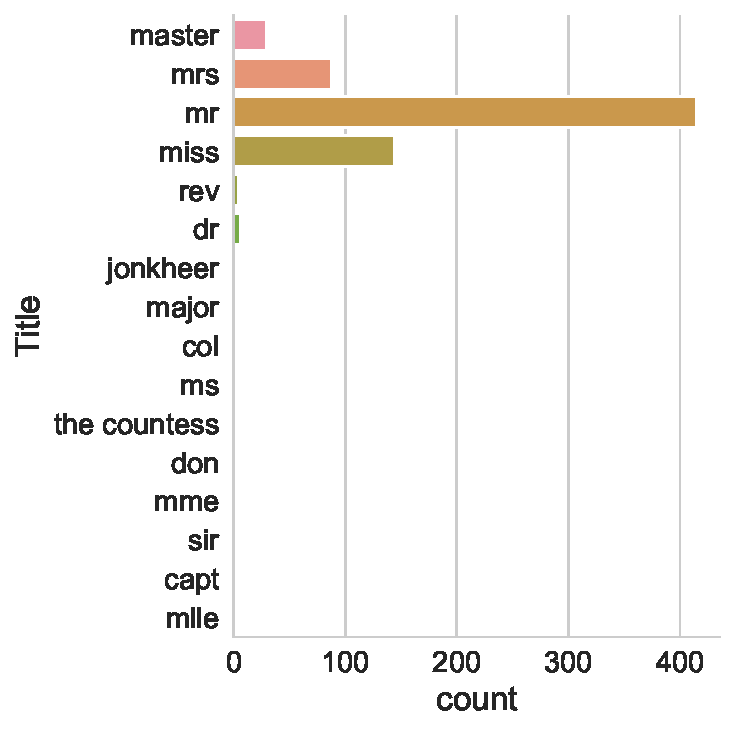
\includegraphics[width=0.5\textwidth]{title_count}
    \caption{Number of occurrences of each title}
    \label{pic:title_count}
\end{figure}

Several titles occurs extremely rarely, the figure \ref{pic:title_belonging_to_class}
shows what \textbf{Pclass} these titles belong to.

\begin{figure}[!ht]
    \centering
    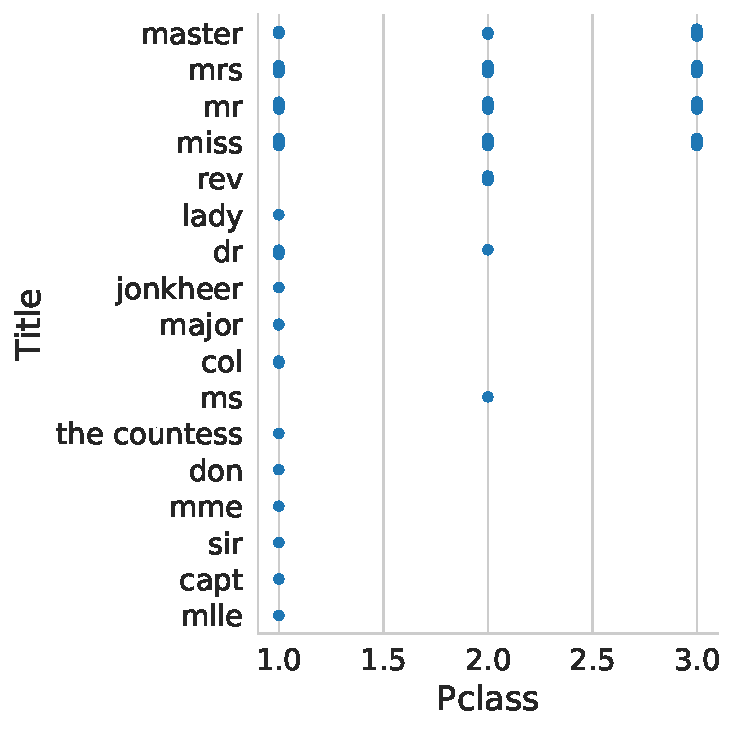
\includegraphics[width=0.5\textwidth]{title_belonging_to_class}
    \caption{\textbf{Title}s belonging to \textbf{Pclass}es}
    \label{pic:title_belonging_to_class}
\end{figure}

People with titles \textit{'rev'}, \textit{'lady'}, \textit{'dr'}, 
\textit{'jonkheer'}, \textit{'major'}, \textit{'col'}, \textit{'ms'}, 
\textit{'the countess'}, \textit{'don'}, \textit{'mme'}, \textit{'sir'}, 
\textit{'capt'}, \textit{'mlle'} belong to the first
or second \textbf{Pclass}, perhaps they are members of the same social 
class. Let's assign them a new \textit{'aristocratic'} category. The
figure \ref{pic:generalized_title_belonging_to_class} shows what 
\textbf{Pclass} the titles with new \textit{'aristocratic'} category 
belong to.

\begin{figure}[!ht]
    \centering
    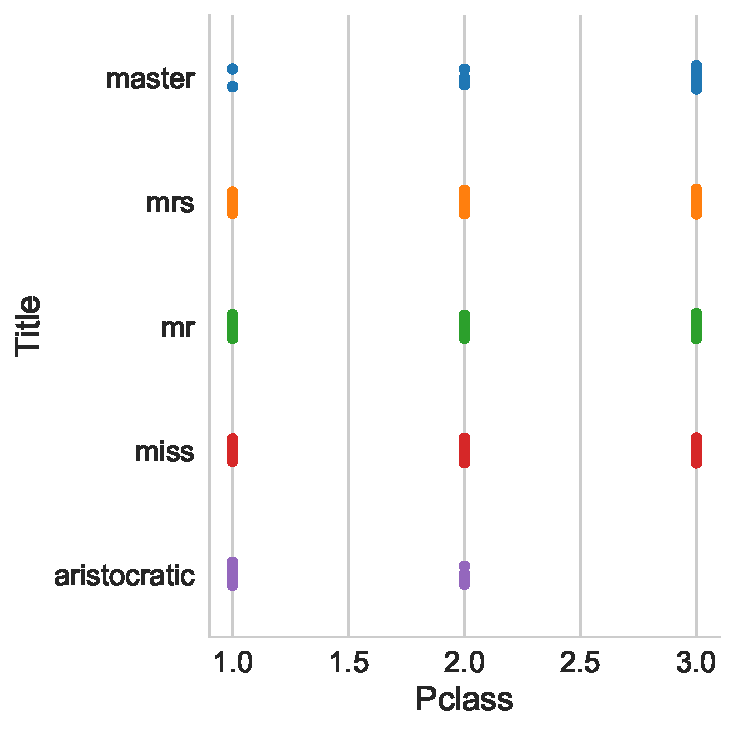
\includegraphics[width=0.5\textwidth]{generalized_title_belonging_to_class}
    \caption{\textbf{Title}s belonging to \textbf{Pclass}es}
    \label{pic:generalized_title_belonging_to_class}
\end{figure}

At last, let's count the proportion of survived passengers for each value
in the new \textbf{Title} feature and the survival rate for men and women
with the title \textit{'aristocratic'}. Figures \ref{pic:title_survival}
and \ref{pic:aristocratic_gender_survival} show respective results.

\begin{figure}[!ht]
    \centering
    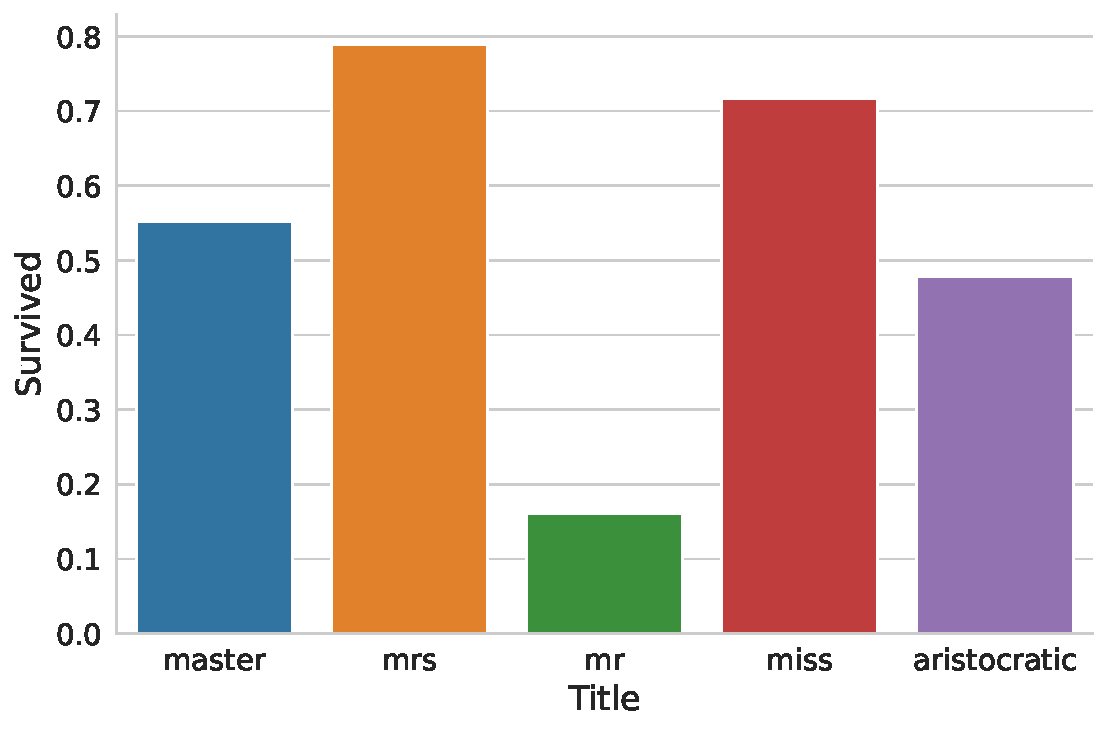
\includegraphics[width=0.5\textwidth]{title_survival}
    \caption{proportion of survived passengers for each value in the new
             \textbf{Title} feature}
    \label{pic:title_survival}
\end{figure}

\begin{figure}[!ht]
    \centering
    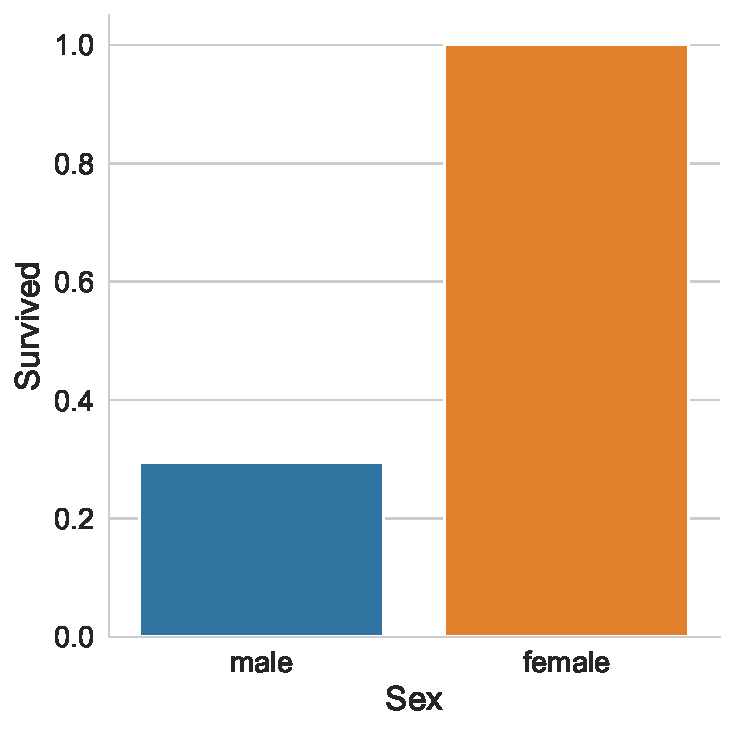
\includegraphics[width=0.5\textwidth]{aristocratic_gender_survival}
    \caption{Survival rate for men and women with the title 
             \textit{'aristocratic'}}
    \label{pic:aristocratic_gender_survival}
\end{figure}

Accordingly to the figure \ref{pic:title_survival} people with titles
\textit{'mrs'}, \textit{'miss'} and \textit{'master'} were most likely 
to survive. \textit{'Master'} is an English honorific for boys and young 
men \cite{english_honorics}. This pattern is consistent with "women and 
children first" protocol. As shown in the figure 
\ref{pic:aristocratic_gender_survival}, for the women and men with 
\textbf{Title} \textit{'aristocratic'} the survival rate is almost the 
same as survival rates for men and women in the entire dataset (see 
\ref{proportion_of_survived_women}).


\section{Sex} \label{section:Sex}
\subsection{Description}
The \textbf{Sex} attribute contains information about the gender of the 
passenger. The table \ref{table:excerpt_from_sex_column} contains excerpt 
from this column. The table \ref{table:sex_characteristics} contains the 
attribute characteristics. The table \ref{table:sex_value_counts} contains 
the number of occurrences of each value.

\begin{table}[!ht]
    \centering
    \caption{Excerpt from the \textbf{Sex} column}
    \begin{tabular}{|l|l|l|l|l|l|}
        \hline
        \textbf{Index} & 788  & 347    & 629  & 734  & 106    \\ \hline
        \textbf{Sex}   & male & female & male & male & female \\ \hline
    \end{tabular}
    \label{table:excerpt_from_sex_column}
\end{table}

\begin{table}[!ht]
    \centering
    \caption{Attribute characteristics}
    \begin{tabular}{|l|l|}
        \hline
        \textbf{Characteristic}   & \textbf{Value} \\ \hline
        Type                      & category       \\ \hline
        Number of values          & 712            \\ \hline
        Number of non-null values & 712            \\ \hline
        Number of unique values   & 2              \\ \hline
        Most frequent value       & male           \\ \hline
    \end{tabular}
    \label{table:sex_characteristics}
\end{table}

\begin{table}[!ht]
    \centering
    \caption{Number of occurrences of each value}
    \begin{tabular}{|l|l|}
        \hline
        \textbf{Value}  & \textbf{Number} \\ \hline
        male            & 461             \\ \hline
        female          & 251             \\ \hline
    \end{tabular}
    \label{table:sex_value_counts}
\end{table}

\subsection{Analysis}
We have already studied this attribute in chapter \ref{chapter:sample_test_set}
"Sample a Test Set". Figures \ref{proportion_of_survived_women} and 
\ref{proportion_of_survived_women_among_pclasses} have shown that in the 
entire dataset and in each \textbf{"Pclass"} there are more female
survivors than males. So, it's very important attribute, and I will
consider other attributes separetely for each gender.

The figure \ref{pic:number_of_men_and_women} shows the number of passengers 
of each gender on board the Titanic. 

\begin{figure}
    \centering
    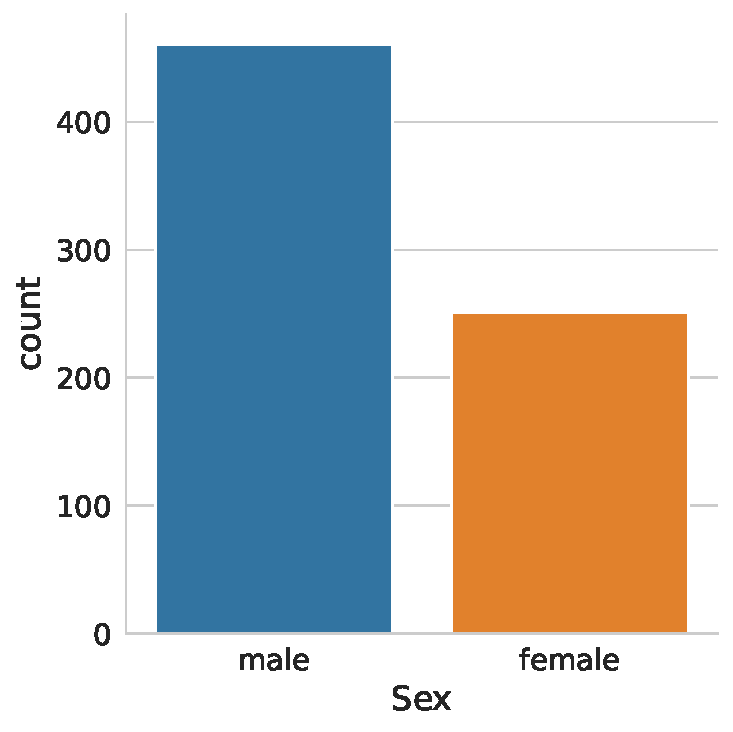
\includegraphics[width=0.5\textwidth]{number_of_men_and_women}
    \caption{Number of men and women on board the Titanic}
    \label{pic:number_of_men_and_women}
\end{figure}

The figure \ref{pic:survial_rate_of_men_and_women} shows the proportion 
of survived men and women in the exploratory set.

\begin{figure}
    \centering
    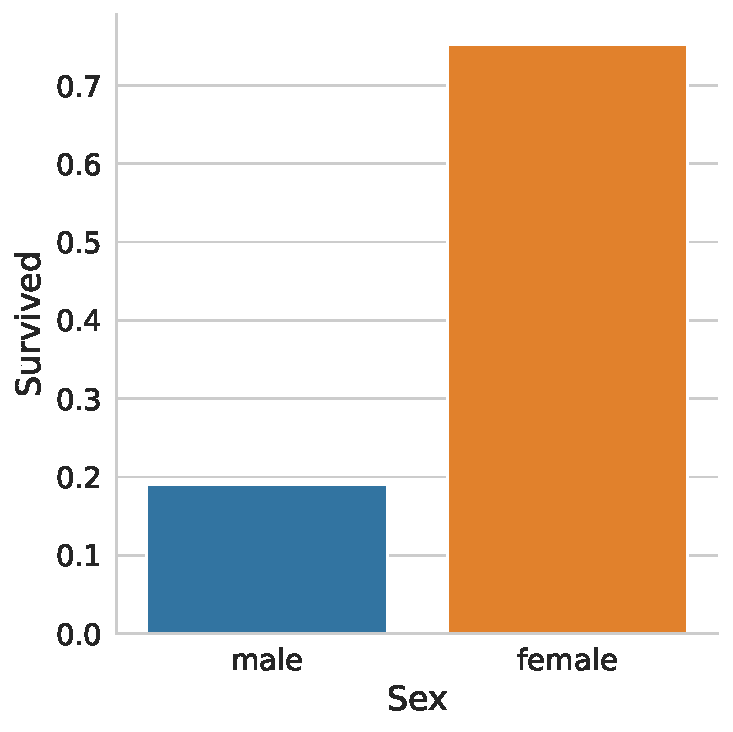
\includegraphics[width=0.5\textwidth]{survial_rate_of_men_and_women}
    \caption{Proportion of survived men and women}
    \label{pic:survial_rate_of_men_and_women}
\end{figure}


\section{Age} \label{section:Age}
\subsection{Description}
The \textbf{Age} attribute contains age of a passenger. The table 
\ref{table:age_head} contains excerpt from attribute's column. The table
\ref{table:age_characteristics} contains the attribute characteristics.

\begin{table}[!ht]
    \centering
    \caption{Excerpt from the \textbf{Age} column}
    \begin{tabular}{|l|l|l|l|l|l|}
        \hline
        \textbf{Index}     & 788 & 347 & 629 & 734  & 106  \\ \hline
        \textbf{Attribute} & 1.0 & NaN & NaN & 23.0 & 21.0 \\ \hline
    \end{tabular}
    \label{table:age_head}
\end{table}

\begin{table}[!ht]
    \centering
    \caption{Attribute characteristics}
    \begin{tabular}{|l|l|}
        \hline
        \textbf{Characteristic}   & \textbf{Value}                  \\ \hline
        Type                      & numerical (float64), continuous \\ \hline
        Number of values          & 712                             \\ \hline
        Number of non-null values & 578                             \\ \hline
        mean                      & 29.781436                       \\ \hline
        std                       & 14.628503                       \\ \hline
        min                       & 0.420000                        \\ \hline
        25\%                      & 21.000000                       \\ \hline
        50\%                      & 28.000000                       \\ \hline
        75\%                      & 38.000000                       \\ \hline
        max                       & 80.000000                       \\ \hline
    \end{tabular}
    \label{table:age_characteristics}
\end{table}

\subsection{Analysis}
At first, let's study the distribution of the \textbf{Age} attribute.
The figures \ref{pic:age_distribution} and \ref{pic:age_ecdf} show the 
histogram with KDE and ECDF respectively.

\begin{figure}[!ht]
    \centering
    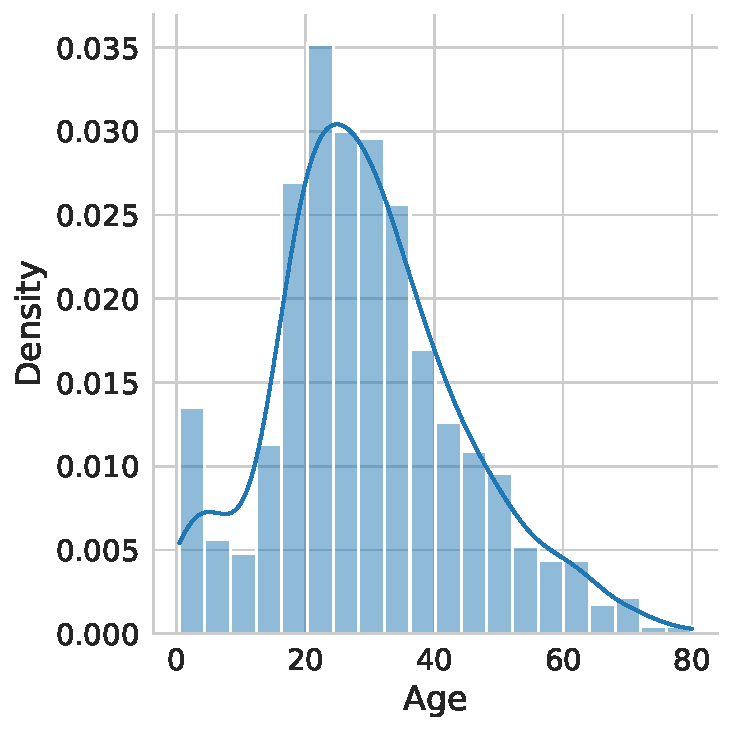
\includegraphics[width=0.5\textwidth]{age_distribution}
    \caption{Histograms of the \textbf{Age} attribute}
    \label{pic:age_distribution}
\end{figure}

\begin{figure}[!ht]
    \centering
    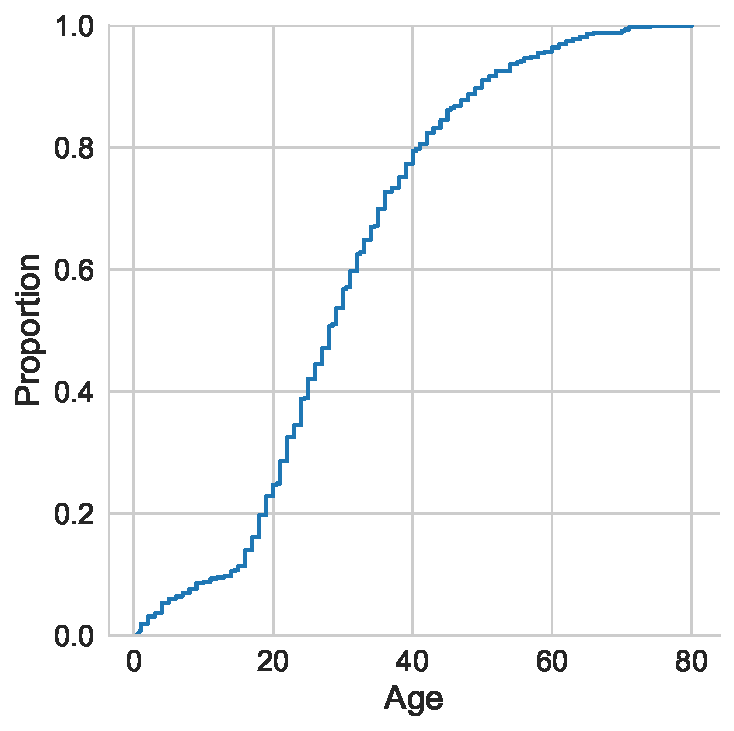
\includegraphics[width=0.5\textwidth]{age_ecdf}
    \caption{ECDF of the \textbf{Age} attribute}
    \label{pic:age_ecdf}
\end{figure}

Obviously, the distribution is skewed and tail-heavy, so we may need to 
do some transformations, such as standardization.

Next, I'm going to test the assumption that the surviving passengers are 
younger. The figure \ref{pic:age_by_survived_cat} illustrates distribution 
of survived and drowned passengers by age. The obvious pattern is not 
visible here.

\begin{figure}[!ht]
    \centering
    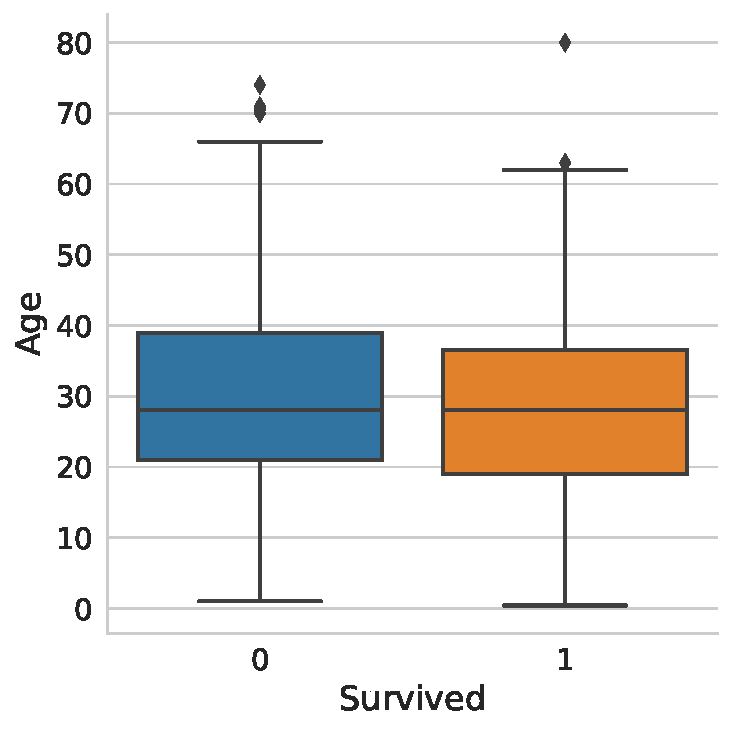
\includegraphics[width=0.5\textwidth]{age_by_survived_cat}
    \caption{Distributions of survived and drowned passengers by age}
    \label{pic:age_by_survived_cat}
\end{figure}

Let's check the distribution of passengers by age in each \textbf{Pclass}.
The corresponding boxplots are shown in the figure \ref{pic:age_by_pclass_cat}.
People from higher socio-economic classes appear to be older.

\begin{figure}[!ht]
    \centering
    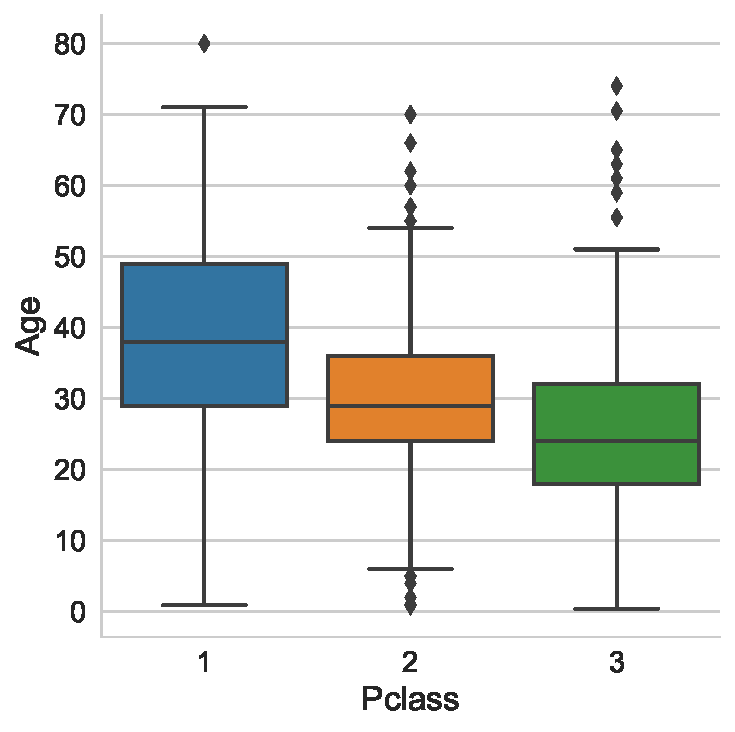
\includegraphics[width=0.5\textwidth]{age_by_pclass_cat}
    \caption{Distributions of passengers by age in each \textbf{Pclass}}
    \label{pic:age_by_pclass_cat}
\end{figure}

At last, let's look on the distributions of representatives of each 
\textbf{Title} by age. The corresponding boxplots are shown in the figure 
\ref{pic:age_by_title_cat}.

\begin{figure}[!ht]
    \centering
    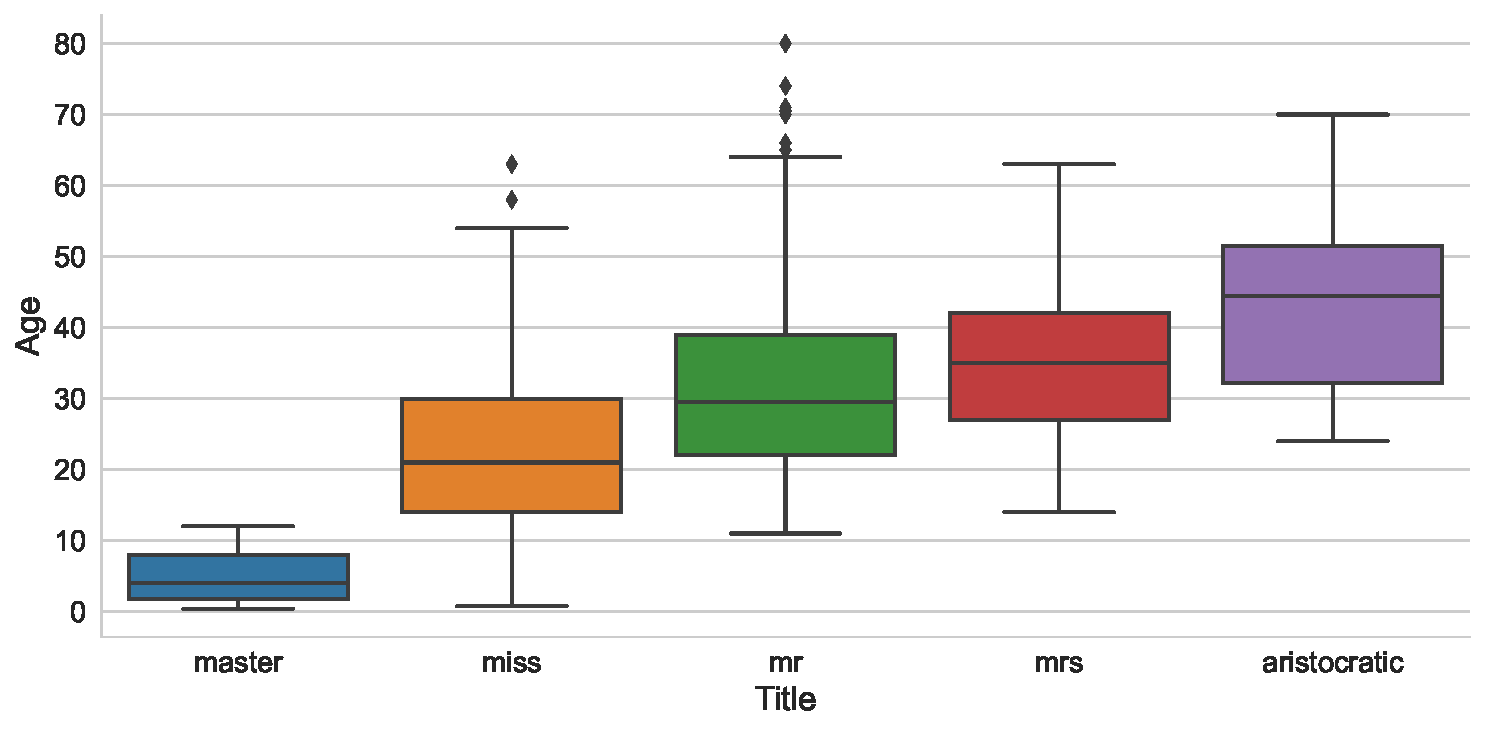
\includegraphics[width=\textwidth]{age_by_title_cat}
    \caption{Distributions of representatives of each title by age}
    \label{pic:age_by_title_cat}
\end{figure}


\section{SibSp} \label{section:SibSp}
\subsection{Description}
The \textbf{SibSp} attribute contains the number of siblings (brother, 
sister, stepbrother, stepsister) or spouses (husband, wife) aboard the 
Titanic. The table \ref{table:sibsp_head} contains excerpt from 
attribute's column. The table \ref{table:sibsp_characteristics} contains
the attribute characteristics.

There is not so many unique values, so let's count number of occurrences 
of each value. The results is shown in the table \ref{table:sibsp_value_counts}.

\begin{table}[!ht]
    \centering
    \caption{Excerpt from the \textbf{SibSp} column}
    \begin{tabular}{|l|l|l|l|l|l|}
        \hline
        \textbf{Index} & 788 & 347 & 629 & 734 & 106 \\ \hline
        \textbf{Value} & 1   & 1   & 0   & 0   & 0   \\ \hline
    \end{tabular}
    \label{table:sibsp_head}
\end{table}

\begin{table}[!ht]
    \centering
    \caption{Number of occurrences of each value}
    \begin{tabular}{|l|l|}
        \hline
        \textbf{Characteristic}   & \textbf{Value}              \\ \hline
        Type                      & numerical (int64), discrete \\ \hline
        Number of values          & 712                         \\ \hline
        Number of non-null values & 712                         \\ \hline
        mean                      & 0.546348                    \\ \hline
        std                       & 1.110283                    \\ \hline
        min                       & 0.000000                    \\ \hline
        25\%                      & 0.000000                    \\ \hline
        50\%                      & 0.000000                    \\ \hline
        75\%                      & 1.000000                    \\ \hline
        max                       & 8.000000                    \\ \hline
    \end{tabular}
    \label{table:sibsp_characteristics}
\end{table}

\begin{table}[!ht]
    \centering
    \caption{Attribute characteristics}
    \begin{tabular}{|l|l|l|l|l|l|l|l|}
        \hline
        \textbf{Value}  & 0   & 1   & 2  & 4  & 3  & 8 & 5 \\ \hline
        \textbf{Number} & 477 & 171 & 25 & 16 & 13 & 5 & 5 \\ \hline
    \end{tabular}
    \label{table:sibsp_value_counts}
\end{table}

\subsection{Analysis}
Let's first examine the distribution of the attribute's values. The
distribution is shown in the figure \ref{pic:sibsp_distribution}. This
distribution is skewed and tail-heave. In truth, it's more like an 
exponential distribution.

\begin{figure}[!ht]
    \centering
    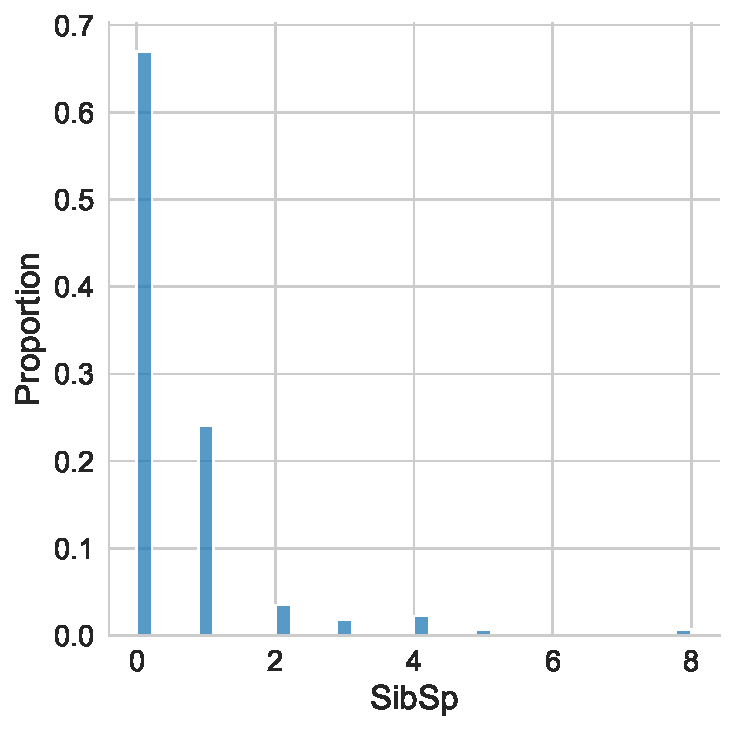
\includegraphics[width=0.5\textwidth]{sibsp_distribution}
    \caption{Distributions of the \textbf{SibSp} attribute's values}
    \label{pic:sibsp_distribution}
\end{figure}

The figure \ref{pic:sibsp_survival_rate} shows the proportion of survived
passengers for each \textbf{SibSp} value. It seems that passengers with
one sibling or spose had more chances to survive.

\begin{figure}[!ht]
    \centering
    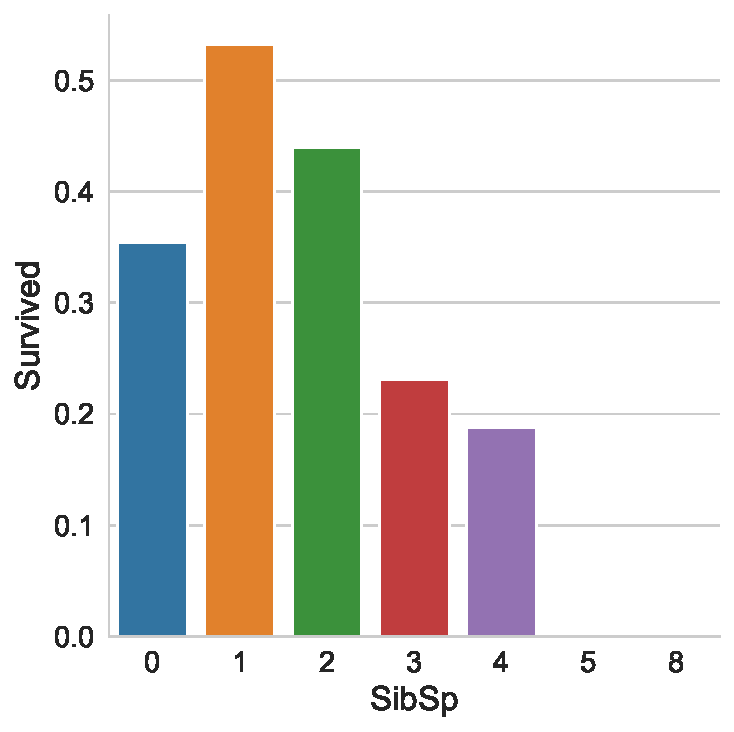
\includegraphics[width=0.5\textwidth]{sibsp_survival_rate}
    \caption{Proportion of survived passengers for each \textbf{SibSp}
             value}
    \label{pic:sibsp_survival_rate}
\end{figure}


\section{Parch} \label{section:Parch}
\subsection{Description}
Attribure description
\textbf{Parch} -- Number of parents or children aboard the Titanic.

\subsection{Analysis}
Attribure Analysis


\section{Ticket} \label{section:Ticket}
\subsection{Description}
Attribure description
\textbf{Ticket} -- Ticket number, for example, A/5 21171.

\subsection{Analysis}
Attribure Analysis


\section{Fare} \label{section:Fare}
\subsection{Description}
Attribure description
\textbf{Fare} -- Passenger fare, for ecample, 71.2833.

\subsection{Analysis}
Attribure Analysis


\section{Cabin} \label{section:Cabin}
\subsection{Description}
Attribure description
\textbf{Cabin} -- Cabin number, for example, C85.

\subsection{Analysis}
Attribure Analysis


\section{Embarked} \label{section:Embarked}
\subsection{Description}
Attribure description
\textbf{Embarked} -- Port of Embarkation:
\begin{itemize}
    \item C = Cherbourg,
    \item Q = Queenstown,
    \item S = Southampton.
\end{itemize}

\subsection{Analysis}
Attribure Analysis